\documentclass[12pt,letterpaper]{standalone}
\usepackage{pgf, tikz}
\usetikzlibrary{arrows, automata}
\usepackage{mwe} % For dummy images 
\usetikzlibrary{positioning}

\begin{document}
	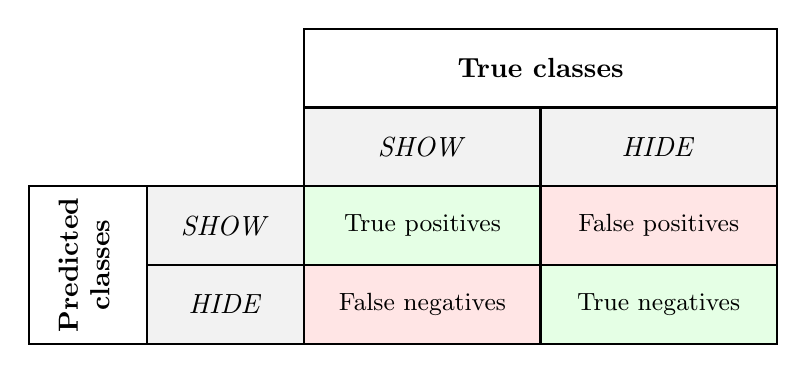
\begin{tikzpicture}
		\draw[thick, fill=red!10] (0,0) rectangle (3,1);
		\draw[thick, fill=green!10] (3,0) rectangle (6,1);
		\draw[thick, fill=green!10] (0,1) rectangle (3,2);
		\draw[thick, fill=red!10] (3,1) rectangle (6,2);
		
		\draw[thick, fill=gray!10]  (-2, 0) rectangle (0, 1);
		\draw[thick, fill=gray!10]  (-2, 1) rectangle (0, 2);
		\draw[thick, fill=gray!10]  (0, 2) rectangle (3, 3);
		\draw[thick, fill=gray!10]  (3, 2) rectangle (6, 3);
		\draw[thick] (-3.5, 0) rectangle (-2, 2);
		\draw[thick] (0, 3) rectangle (6, 4);
		
		\node() at (3, 3.5) {\textbf{True classes}};
		\node[rotate=90] () at (-3.0, 1) {\textbf{Predicted}};
		\node[rotate=90] () at (-2.6, 1) {\textbf{classes}};
		
		\node () at (-1, 1.5) {\textit{SHOW}};
		\node () at (-1, 0.5) {\textit{HIDE}};
		\node () at (1.5, 2.5) {\textit{SHOW}};
		\node () at (4.5, 2.5) {\textit{HIDE}};
		
		\node () at (1.5, 1.5) {\small True positives};
		\node () at (1.5, 0.5) {\small False negatives};
		\node () at (4.5, 1.5) {\small False positives};
		\node () at (4.5, 0.5) {\small True negatives};
	\end{tikzpicture}
\end{document}